\documentclass[10pt]{beamer}
\usetheme{CambridgeUS}
\usepackage[utf8]{inputenc}
\usepackage[spanish]{babel}
\usepackage{amsmath}
\usepackage{amsfonts}
\usepackage{amssymb}
\usepackage{graphicx}
\usepackage{ragged2e}
\usepackage{multicol}
\usepackage{multirow, array}
\author{Kevin García - Alejandro Vargas}
\title{Gráfico de Control Multivariantes}
%\setbeamercovered{transparent} 
%\setbeamertemplate{navigation symbols}{} 
%\logo{} 
%\institute{} 
%\date{} 
%\subject{} 
\justifying
\begin{document}

\begin{frame}[plain]
\maketitle
\end{frame}

\begin{frame}{Contenido}
\tableofcontents
\end{frame}

\section{Introducción}
\begin{frame}{Introducción}

\end{frame}

\section{Antecedentes}
\begin{frame}{Antecedentes}

\end{frame}

\section{Descripción de la metodología}
\begin{frame}{Metodología}

\end{frame}

\section{Caso ilustrativo}
\begin{frame}{Ejemplo}

\end{frame}


\section{Conclusiones}
\begin{frame}{Conclusiones}

\end{frame}

\section{Bibliografía}
\begin{frame}
  \frametitle{Bibliografía}
  
\nocite{A0,ControlR}
  
  \bibliographystyle{plain}
  \bibliography{references}
\end{frame}

\section{Anexos}
\begin{frame}{Anexos}
\begin{figure}[h!]
  \centering
  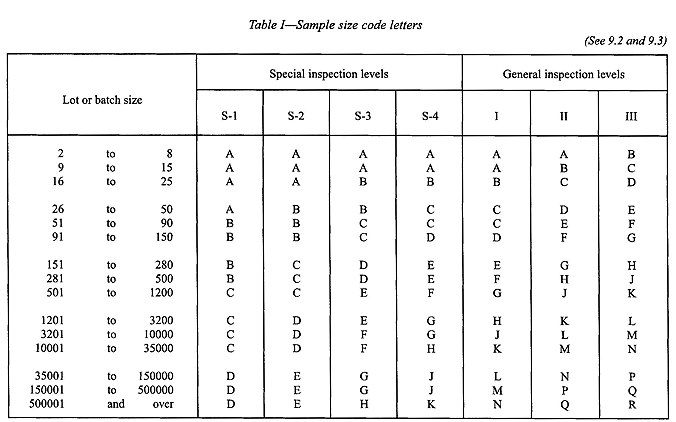
\includegraphics[scale=0.55]{FigurasUV/letra.png}
  \caption{Letra código del plan}
\end{figure}
\end{frame}


\end{document}
